\documentclass[
	10pt,								% globale Schriftgröße
	parskip=half-,						% setzt Absatzabstand hoch
	paper=a4,							% Format
	english,ngerman,					% lädt Sprachpakete
	]{scrartcl}							% Dokumentenklasse

% //////////////////// Pakete laden ////////////////////
\usepackage[fleqn]{amsmath}
\usepackage[fleqn]{mathtools}
\usepackage{amssymb}			% mathematische symbole, für \ceckmarks
\usepackage{amsthm}				% für proof
\usepackage{mathrsfs}			% für \mathscr
\usepackage{latexsym}
\usepackage{marvosym}				% für Lightning

\usepackage{fontspec} 			% funktioniert nur mit den neueren Compilern z.B. XeLaTeX
\usepackage{microtype}			% für bessere Worttrennung
\usepackage[ngerman]{babel} 	% Spracheinstellung
\usepackage{lmodern}			% verändert verwendete Schriftart, damit sie weniger pixelig ist

\usepackage{verbatim}
\usepackage{listings}			% Für Quellcode

\usepackage{graphicx}
\usepackage{tabularx}			% für Tabellen mit gleicher Spaltenbreite und automatischen Umbrüchen
\usepackage{fullpage}
\usepackage{multirow}			% für multirow in tabulars
\usepackage{rotate}
\usepackage[cmyk,table]{xcolor} % um Farben zu benutzen, kann mehr als das Paket color
\usepackage[					% Verlinkungen
	colorlinks,					% farbige Schrift, statt farbiger Rahmen
	linktocpage,				% verlinkt im Abb.Verzeichnis Seitenzahl statt Bildunterschrift
	linkcolor=blue				% setzt Farbe der Links auf blau
	]{hyperref}					% nur für digitale Anwendungen, url = "http://www.example.com"
\usepackage{url}				% für Webadressen wie e-mail usw.: "\url{http://www.example.com}"

\usepackage{enumerate}			% für versch. Aufzählungezeichen wie z.B. a)
\usepackage{xspace}				% folgt ein Leerzeichen nach einem \Befehl, wird es nicht verschluckt.
\usepackage{cancel}				% für das Durchstreichen u.a. in Matheformeln mit \cancel
\usepackage{float}              % zum Forcieren der Position von figure-Umgebungen

% zum Zeichnen (u.a. von Graphen)
\usepackage{fp}
\usepackage{tikz}
\usetikzlibrary{tikzmark}			% für \tikzmark{toRemember}
\usetikzlibrary{positioning}	% verbesserte Positionierung der Knoten
\usetikzlibrary{automata}		% für Automaten (GTI)
\usetikzlibrary{arrows}
\usetikzlibrary{shapes}
\usetikzlibrary{decorations.pathmorphing}
\usetikzlibrary{decorations.pathreplacing}
\usetikzlibrary{decorations.shapes}
\usetikzlibrary{decorations.text}

% //////////////////// Syntaxhighlighting ////////////////////
\lstloadlanguages{Python, Haskell, [LaTeX]TeX, Java}
\lstset{
   basicstyle=\footnotesize\ttfamily,	% \scriptsize the size of the fonts that are used for the code
   backgroundcolor = \color{bgcolour},	% legt Farbe der Box fest
   breakatwhitespace=false,	% sets if automatic breaks should only happen at whitespace
   breaklines=true,			% sets automatic line breaking
   captionpos=t,				% sets the caption-position to bottom, t for top
   commentstyle=\color{codeblue}\ttfamily,% comment style
   frame=single,				% adds a frame around the code
   keepspaces=true,			% keeps spaces in text, useful for keeping indentation
							% of code (possibly needs columns=flexible)
   keywordstyle=\bfseries\ttfamily\color{codepurple},% keyword style
   numbers=left,				% where to put the line-numbers;
   							% possible values are (none, left, right)
   numberstyle=\tiny\color{codegreen},	% the style that is used for the line-numbers
   numbersep=5pt,			% how far the line-numbers are from the code
   stepnumber=1,				% nummeriert nur jede i-te Zeile
   showspaces=false,			% show spaces everywhere adding particular underscores;
							% it overrides 'showstringspaces'
   showstringspaces=false,	% underline spaces within strings only
   showtabs=false,			% show tabs within strings adding particular underscores
   flexiblecolumns=false,
   tabsize=1,				% the step between two line-numbers. If 1: each line will be numbered
   stringstyle=\color{orange}\ttfamily,	% string literal style
   numberblanklines=false,				% leere Zeilen werden nicht mitnummeriert
   xleftmargin=1.2em,					% Abstand zum linken Layoutrand
   xrightmargin=0.4em,					% Abstand zum rechten Layoutrand
   aboveskip=2ex, 
}

\lstdefinestyle{py}{
   language=Python,
}
\lstdefinestyle{hs}{
   language=Haskell,
}
\lstdefinestyle{tex}{
	language=[LaTeX]TeX,
	escapeinside={\%*}{*)},     % if you want to add LaTeX within your code
	texcsstyle=*\bfseries\color{blue},% hervorhebung der tex-Schlüsselwörter
	morekeywords={*,$,\{,\},\[,\],lstinputlisting,includegraphics,
	rowcolor,columncolor,listoffigures,lstlistoflistings,
	subsection,subsubsection,textcolor,tableofcontents,colorbox,
	fcolorbox,definecolor,cellcolor,url,linktocpage,subtitle,
	subject,maketitle,usetikzlibrary,node,path,addbibresource,
	printbibliography},% if you want to add more keywords to the set
     numbers=none,
     numbersep=0pt,
     xleftmargin=0.4em,
}

\lstdefinestyle{java}{
	language=Java,
	extendedchars=true,		% lets you use non-ASCII characters;
   						% for 8-bits encodings only, does not work with UTF-8
}

\lstdefinelanguage[x64]{Assembler}     % add a "x64" dialect of Assembler
   [x86masm]{Assembler} % based on the "x86masm" dialect
   % with these extra keywords:
   {morekeywords={CDQE,CQO,CMPSQ,CMPXCHG16B,JRCXZ,LODSQ,MOVSXD, %
                  POPFQ,PUSHFQ,SCASQ,STOSQ,IRETQ,RDTSCP,SWAPGS, %
                  rax,rdx,rcx,rbx,rsi,rdi,rsp,rbp, %
                  r8,r8d,r8w,r8b,r9,r9d,r9w,r9b}
}					% for 8-bits encodings only, does not work with UTF-8

\lstdefinestyle{c}{
	language=c,
	extendedchars=true,		% for 8-bits encodings only, does not work with UTF-8
}

% //////////////////// eigene Kommandos ////////////////////
\newcommand\FU{Freie Universität Berlin\xspace}% benötigt package xspace
\newcommand\gdw{g.\,d.\,w.\xspace}
\newcommand\oBdA{o.\,B.\,d.\,A.\xspace}
\newcommand{\Eu}{\texteuro}
\newcommand\N{\mathbb{N}\xspace}
\newcommand\Q{\mathbb{Q}\xspace}
\newcommand\R{\mathbb{R}\xspace}
\newcommand\Z{\mathbb{Z}\xspace}
\newcommand\ohneNull{\ensuremath{\backslash\lbrace 0\rbrace}}% \{0}
\let\dhALT\dh	% Schreibt Befehl \dh in \dhALT um
\renewcommand\dh{d.\,h.\xspace}	%renew überschreibt command \dh
\newcommand\Bolt{\;\text{\LARGE\raisebox{-0.3em}{\Lightning}\normalsize}\xspace}% Blitz
\newcommand\zz{\ensuremath{\raisebox{+0.25ex}{Z}% zu zeigen
			\kern-0.4em\raisebox{-0.25ex}{Z}%
			\;\xspace}}
\newcommand{\from}{\ensuremath{\colon}}
\newcommand{\floor}[1]{\lfloor{#1}\rfloor}
\newcommand{\ceil}[1]{\lceil{#1}\rceil}
 \renewcommand{\L}{\ensuremath{\mathcal{L}}\xspace}
 \renewcommand{\P}{\ensuremath{\mathcal{P}}\xspace}
 \newcommand{\NL}{\ensuremath{\mathcal{N}\kern-0.2em\mathcal{L}}\xspace}
 \newcommand{\NP}{\ensuremath{\mathcal{NP}}\xspace}

% //////////////////// Mathefunktionen ////////////////////
\DeclareMathOperator{\Landau}{\mathcal{O}}
\DeclareMathOperator{\True}{True}
\DeclareMathOperator{\False}{False}

% //////////////////// eigene Theoreme ////////////////////
\newtheorem{theorem}{Satz}
\newtheorem{corollary}[theorem]{Folgerung}
\newtheorem{lemma}[theorem]{Lemma}
\newtheorem{observation}[theorem]{Beobachtung}
\newtheorem{definition}[theorem]{Definition}
\newtheorem{Literatur}[theorem]{Literatur}
% konfiguriert proof
\makeatletter
\newenvironment{Proof}[1][\proofname]{\par
  \pushQED{\qed}%
  \normalfont \topsep6\p@\@plus6\p@\relax
  \trivlist
  \item[\hskip\labelsep
%         \itshape
        \bfseries
    #1\@addpunct{.}]\ignorespaces
}{%
  \popQED\endtrivlist\@endpefalse
}
\makeatother

% //////////////////// eigene Farben ////////////////////
\let\definecolor=\xdefinecolor
\definecolor{FUgreen}{RGB}{153,204,0}
\definecolor{FUblue}{RGB}{0,51,102}

\definecolor{middlegray}{rgb}{0.5,0.5,0.5}
\definecolor{lightgray}{rgb}{0.8,0.8,0.8}
\definecolor{orange}{rgb}{0.8,0.3,0.3}
\definecolor{azur}{rgb}{0,0.7,1}
\definecolor{yac}{rgb}{0.6,0.6,0.1}
\definecolor{Pink}{rgb}{1,0,0.6}

\definecolor{bgcolour}{rgb}{0.97,0.97,0.97}
\definecolor{codegreen}{rgb}{0,0.6,0}
\definecolor{codegray}{rgb}{0.35,0.35,0.35}
\definecolor{codepurple}{rgb}{0.58,0,0.82}
\definecolor{codeblue}{rgb}{0.4,0.5,1}

% //////////////////// eigene Settings ////////////////////

\textheight = 230mm		% Höhe des Satzspiegels / Layouts
\footskip = 10ex			% Abstand zw. Fußzeile und Grundlinie letzter Textzeile
\parindent 0pt			% verhindert Einrückung der 1. Zeile eines Absatzes
\setkomafont{sectioning}{\rmfamily\bfseries}% setzt Ü-Schriften in Serifen, {disposition}											% bindet Header ein (WICHTIG)
\usepackage{graphicx}
\usepackage{amsmath}
\usepackage{amssymb}
\usepackage{fancyvrb}

\newcommand{\dozent}{Prof. R. Rojas}					% <-- Names des Dozenten eintragen
\newcommand{\projectNo}{7}
\newcommand{\veranstaltung}{Mustererkennung}
\newcommand{\semester}{WS17/18}
\newcommand{\studenten}{Boyan Hristov, Nedeltscho Petrov}
% /////////////////////// BEGIN DOKUMENT /////////////////////////


\begin{document}
% /////////////////////// BEGIN TITLEPAGE /////////////////////////
\begin{titlepage}
	\subject{\dozent}
	\title{\veranstaltung, \semester}
	\subtitle{\Large Übungsblatt \projectNo\\ \large\vspace{1ex} }
	\author{\studenten}
	\date{\normalsize \today}
\end{titlepage}

\maketitle								% Erstellt das Titelblatt
\vspace*{-9cm}							% rückt Logo an den oberen Seitenrand
\makebox[\dimexpr\textwidth+1cm][r]{	%rechtsbündig und geht rechts 1cm über Layout hinaus
	
\includegraphics[width=0.4\textwidth]{src/fu_logo} % fügt FU-Logo ein
}
% /////////////////////// END TITLEPAGE /////////////////////////

\vspace{7cm}							% Abstand
\rule{\linewidth}{0.8pt}				% horizontale Linie										% erstellt die Titelseite


Link zum Git Repository: \url{https://github.com/BoyanH/FU-MachineLearning-17-18/tree/master/Solutions/Homework\projectNo}

\section*{Logistische Regression}

\section*{Ausgabe des Programms und damit Score}

\begin{lstlisting}
Score: 0.9294245385450597
[[541  42]
 [ 23 315]]
Score from sklearn: 0.9370249728555917
\end{lstlisting}

\section*{Absolute Wert von Log Likelihood während der Iteration}
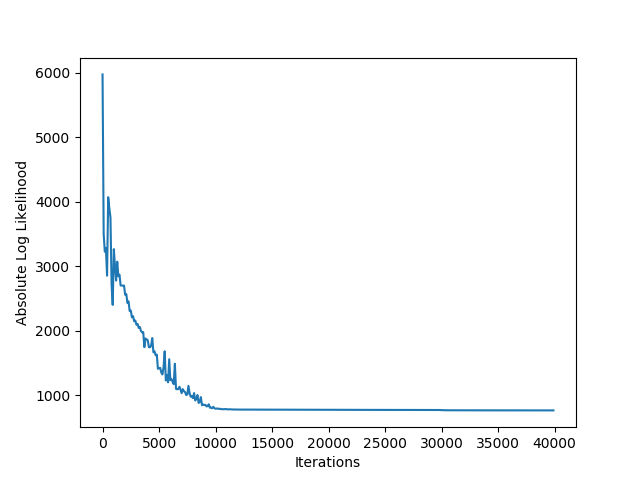
\includegraphics[height=8cm]{./ll_over_time.png}

\section*{Wie kann man eine Klasse bevorzugen}

Wir können den ersten Koeffizient in dem Gewichtsvektor etwas ändern. Falls wir es höher setzen, werden wir
die positive Klasse bevorzugen und umgekehrt.

\section*{Erklärung des Codes}

\section*{Transformation}

Wir normalisieren immer die Daten, in dem Wir je Feature duch den Varianz aller solchen Features teilen.
Diese transform Methode wird vor dem Fitting und auch vor je Vorhersage gemacht. Weiter fügen wir hier auch
die Spalte mit 1. ein.

\begin{lstlisting}[style=py]
    def transform(self, X, y):

        # feature_means = X.sum(0) / len(X[0])
        # X_t = X.T
        # variance = [((X_t[i] - feature_means[i])**2).sum() for i in range(len(X_t))]

        # numpy does it more effectively and normalized
        self.transformation_vector = np.var(X, axis=0)
        X = X / self.transformation_vector

        ones = np.ones((len(X), 1), dtype=np.float64)
        X = np.append(ones, X, axis=1)

        return X, y
\end{lstlisting}

\section*{Fit Methode}

In der Fit Methode versuchen wir, die Likelihood zu maximieren. Das machen wir anhand der Gradientensteigerung
der Log-likelihood. Um das zu approximieren, nutzt man ein learning rate, da man von den Gradientensteigerung nur
erfährt, in welcher Richtung unsere Lösung sich befindet. Die Implementierung benutzt für die Berechnung der
Steigerung die in der Vorlesung besprochene Formeln, deswegen ist hier die Lernrate interessanter.

Da wir mit einer statischen Lernrate etwas schlechtere
Ergbebnisse (um circa 2% schlechter) bekommen haben, haben wir die "bold driver" Methode benutzt (aber für unser Datensatz
etwas angepasst). Laut die Methode, muss man jedes mal, wenn man ein schlechteres Ergebniss bekommt, die Lernrate
halbieren und das vorherige Gewichtsvektor nehmen. Sonst darf man die lernrate um 5% erhöhen. Bei uns waren das
aber 3% kleinere Lernrate bei einer höheren Fehler und 0.03% höhere Lernrate sonst.

\begin{lstlisting}[style=py]
def fit(self, X, y, iterations, plot):
        features_len = len(X[0])
        self.beta = np.zeros(features_len, dtype=np.float64)
        log_error_over_time = []

        last_log_error = float('inf')
        current_learning_rate = self.learn_rate

        for i in range(iterations):
            weighted = X.dot(self.beta)
            probabilities = LogisticRegression.sigmoid(weighted)
            directions = y - probabilities
            gradient = X.T.dot(directions)

            self.learn_rate = self.learn_rate / 2
            self.beta = self.beta + current_learning_rate*gradient

            if i % 100 == 0:
                current_log_error = abs(self.get_log_likelihood(X, y))

                if current_log_error < last_log_error:
                    current_learning_rate += current_learning_rate * 0.0003  # increase by 0.03%
                else:
                    self.beta = last_beta
                    current_learning_rate -= current_learning_rate * 0.03 # decrease by 3%

                last_log_error = current_log_error
                last_beta = np.copy(self.beta)
\end{lstlisting}

\section*{Predict Methode}

Die predict Methode ist ganz simpel. Deswegen wäre hier auch interessant die get\_probability Methode,
die haben wir aber 1 zu 1 aus der Vorlesung genommen.
\begin{lstlisting}[style=py]
    def predict_single(self, x):
        return 1 if self.get_probability(x, 1) > 0.5 else 0

    def get_probability(self, x, y):
        return 1 / (1 + math.exp((-y * self.beta).T.dot(x)))
\end{lstlisting}

\section*{Analyse booleschen Funktionen}

\section*{Output des Programs}

\begin{lstlisting}
beta and vs or: [ 0.11601896  0.53124725  0.53124725 -1.12376802]
transformed X and vs or: [[ 1.  0.  0.  0.]
 [ 1.  0.  4.  0.]
 [ 1.  4.  0.  0.]
 [ 1.  4.  4.  4.]
 [ 1.  0.  0.  0.]
 [ 1.  0.  4.  4.]
 [ 1.  4.  0.  4.]
 [ 1.  4.  4.  4.]]
Predicted: [1, 1, 1, 0, 1, 0, 0, 0]; Expected: [ 1.  1.  1.  1.  0.  0.  0.  0.]
beta and vs xor: [ 0.0795093   0.09251593  0.09251593 -0.29707532]
transformed X and vs xor: [[ 1.          0.          0.          0.        ]
 [ 1.          0.          4.          0.        ]
 [ 1.          4.          0.          0.        ]
 [ 1.          4.          4.          4.26666667]
 [ 1.          0.          0.          0.        ]
 [ 1.          0.          4.          4.26666667]
 [ 1.          4.          0.          4.26666667]
 [ 1.          4.          4.          0.        ]]
Predicted: [1, 1, 1, 0, 1, 0, 0, 1]; Expected: [ 1.  1.  1.  1.  0.  0.  0.  0.]
beta or vs xor: [-0.18989504 -0.115224   -0.115224    0.26844163]
transformed X or vs xor: [[ 1.          0.          0.          0.        ]
 [ 1.          0.          4.          4.26666667]
 [ 1.          4.          0.          4.26666667]
 [ 1.          4.          4.          4.26666667]
 [ 1.          0.          0.          0.        ]
 [ 1.          0.          4.          4.26666667]
 [ 1.          4.          0.          4.26666667]
 [ 1.          4.          4.          0.        ]]
Predicted: [0, 1, 1, 1, 0, 1, 1, 0]; Expected: [ 1.  1.  1.  1.  0.  0.  0.  0.]
\end{lstlisting}

\section*{Analyse}

Bei AND vs OR sehen wir, dass das Endergebniss die entschedentste Rolle hat mit Koeffizient von $-1.124$. Das klingt auch
logisch, da die AND Funktion seltener ein Wert von 1 zurückgibt als ein Wert von 0.
$ 1 - \frac{1}{1 + e^{-(0.11601896 -1.124*4)}}  \approx 98.7\%$, dass es keine AND ist, wenn die Funktion 1 zurückgibt.
Die zwei Eingabewerte haben je ein Einfluss von $ 1 - \frac{1}{1 + e^{-(0.11601896 + 0.53124725*4)}}  \approx 9.6\%$,
dass es eine OR Funktion ist. \\\\

Wir können sehen, dass unsere Theorie stimmt, da das Algorithmus bei allen Eingaben mit Endergebniss 1 eine OR
Funktion vorhergesehen haben. Das kann man auch ausrechen:
$ 1 - \frac{1}{1 + e^{-(0.11601896 +2*4*0.53124725 -1.124*4)}}  \approx 53.2\%$ dass es eine AND Funktion ist. \\\\

Bei AND vs XOR sieht man wieder, dass das Endergebniss beides in der Normalisierung und auch bei dem Beta-Koeffizeint
das größte Einfluss hat. Das ist so, da 1 XOR 0 = 1, 0 XOR 1 = 1, wobei AND bei den gleichen Werten 0 zurückgibt.
Der Koeffizient ist aber nicht so groß wie bei AND vs OR, da 1 XOR 1 = 0 und 1 AND 1 = 1, also das Gegenbeispiel.
Wir sehen aber wieder, dass das Algorithmus immer bei Endergebniss 1 eine XOR vorhersagt. \\\\

OR und XOR kann man nur anhand von dem letzten Sample von dem Datensatz unterscheiden. Also
1 OR 1 = 1 und 1 XOR 1 = 0. Andere Eingaben liefern gleiche Ausgaben. Deswegen, ein Endergebniss von 1 wurde
eine OR bevorzugen (Koeffizient 0.26844163). Wir sehen auch, dass das Algorithmus nur bei diesen Eingaben
bei beiden Klassen keine Fehler macht.

\section*{Vollständiges Code}

\section*{LogisticRegression.py}

\begin{lstlisting}[style=py]
from Classifier import Classifier
import numpy as np
import math
from matplotlib import pyplot as plt
import os


class LogisticRegression(Classifier):
    # def __init__(self, X_train, y_train, learn_rate=1e-3):
    def __init__(self, X_train, y_train, learn_rate=1e-3, iterations=40000, plot=False):
        self.beta = None
        self.transformation_vector = None
        self.learn_rate = learn_rate
        X, y = self.transform(X_train, y_train)
        self.fit(X, y, iterations, plot)

    @staticmethod
    def sigmoid(weighted):
        return 1 / (1 + np.exp(-weighted))

    def transform(self, X, y):

        # feature_means = X.sum(0) / len(X[0])
        # X_t = X.T
        # variance = [((X_t[i] - feature_means[i])**2).sum() for i in range(len(X_t))]

        # numpy does it more effectively and normalized
        self.transformation_vector = np.var(X, axis=0)
        X = X / self.transformation_vector

        # add ones
        ones = np.ones((len(X), 1), dtype=np.float64)
        X = np.append(ones, X, axis=1)

        return X, y

    def fit(self, X, y, iterations, plot):
        features_len = len(X[0])
        self.beta = np.zeros(features_len, dtype=np.float64)
        log_error_over_time = []

        last_log_error = float('inf')
        current_learning_rate = self.learn_rate

        for i in range(iterations):
            weighted = X.dot(self.beta)
            probabilities = LogisticRegression.sigmoid(weighted)
            directions = y - probabilities
            gradient = X.T.dot(directions)

            # Bold driver technique
            # If error was actually larger (overshooting) use previous weight vector
            # and decrease learning rate by 50%; otherwise increase learn rate by 5%

            # self.beta = self.beta + (self.learn_rate / (2**(i/5000)))*gradient
            self.learn_rate = self.learn_rate / 2
            self.beta = self.beta + current_learning_rate*gradient

            if i % 100 == 0:
                current_log_error = abs(self.get_log_likelihood(X, y))

                if current_log_error < last_log_error:
                    current_learning_rate += current_learning_rate * 0.0003  # increase by 0.03%
                else:
                    self.beta = last_beta
                    current_learning_rate -= current_learning_rate * 0.03 # decrease by 3%

                last_log_error = current_log_error
                last_beta = np.copy(self.beta)

                if plot:
                    log_error_over_time.append(current_log_error)

        if plot:
            plt.ylabel('Absolute Log Likelihood')
            plt.xlabel('Iterations')
            plt.plot([i for i in range(0, iterations, 100)], log_error_over_time)
            plt.savefig(os.path.join(os.path.dirname(__file__), 'll_over_time.png'))

    def predict(self, X):
        X = X / self.transformation_vector
        # add ones
        ones = np.ones((len(X), 1), dtype=np.float64)
        X = np.append(ones, X, axis=1)
        return list(map(lambda x: self.predict_single(x), X))

    def get_integrated_error(self, X, y):

        data_len = len(y)
        get_integrated_error_per_data_point = np.vectorize(
            lambda idx: y[idx]*X[idx]*(1 - self.get_probability(X[idx], y[idx])),
            signature='()->(m)')
        integrated_errors = get_integrated_error_per_data_point(range(data_len))

        return integrated_errors.sum(0)

    def get_probability(self, x, y):
        try:
            return 1 / (1 + math.exp((-y * self.beta).T.dot(x)))
        except:
            return 0

    def predict_single(self, x):
        return 1 if self.get_probability(x, 1) > 0.5 else 0

    def get_log_likelihood(self, X, y):
        weighted = X.dot(self.beta)
        return np.sum(y * weighted - np.log(1 + np.exp(weighted)))

\end{lstlisting}

\section*{LogisticRegressionDemo.py}

\begin{lstlisting}[style=py]
from sklearn.linear_model import LogisticRegression as LRSKL
import numpy as np
from Parser import get_data_set
from LogisticRegression import LogisticRegression

X_train, X_test, y_train, y_test = get_data_set(1)
lr = LogisticRegression(X_train, y_train, plot=True)
score = lr.score(X_test, y_test)
print('Score: {}'.format(score))
print(lr.confusion_matrix(X_test, y_test))

sklearn_lr = LRSKL()
sklearn_lr.fit(X_train, y_train)
predictions = sklearn_lr.predict(X_test)
score_sklearn = np.mean(predictions == y_test)
print('Score from sklearn: {}'.format(score_sklearn))

\end{lstlisting}

\section*{bool\_func\_analysis.py}

\begin{lstlisting}[style=py]
import os
import numpy as np
import pandas as pd
from LogisticRegression import LogisticRegression
from Parser import extract_classes_from_data_set


file_name = os.path.join(os.path.dirname(__file__), './Dataset/boolfunc.data')
data = np.array(pd.read_csv(file_name, header=None).as_matrix())
X = np.array(data[:,:-1], dtype=np.float64)
y = data[:,-1]

and_or_X, and_or_y = extract_classes_from_data_set(X, y, ['and', 'or'])
and_or_y = np.array([1 if x == 'and' else 0 for x in and_or_y], dtype=np.float64)
lr_and_or = LogisticRegression(and_or_X, and_or_y, iterations=1000)
print('beta and vs or: {}'.format(lr_and_or.beta))
print('transformed X and vs or: {}'.format(lr_and_or.transform(and_or_X, and_or_y)[0]))
print('Predicted: {}; Expected: {}'.format(lr_and_or.predict(and_or_X), and_or_y))

and_xor_X, and_xor_y = extract_classes_from_data_set(X, y, ['and', 'xor'])
and_xor_y = np.array([1 if x == 'and' else 0 for x in and_xor_y], dtype=np.float64)
lr_and_xor = LogisticRegression(and_xor_X, and_xor_y, iterations=1000)
print('beta and vs xor: {}'.format(lr_and_xor.beta))
print('transformed X and vs xor: {}'.format(lr_and_xor.transform(and_xor_X, and_xor_y)[0]))
print('Predicted: {}; Expected: {}'.format(lr_and_xor.predict(and_xor_X), and_xor_y))

or_xor_X, or_xor_y = extract_classes_from_data_set(X, y, ['or', 'xor'])
or_xor_y = np.array([1 if x == 'or' else 0 for x in or_xor_y], dtype=np.float64)
lr_or_xor = LogisticRegression(or_xor_X, or_xor_y, iterations=1000)
print('beta or vs xor: {}'.format(lr_or_xor.beta))
print('transformed X or vs xor: {}'.format(lr_or_xor.transform(or_xor_X, or_xor_y)[0]))
print('Predicted: {}; Expected: {}'.format(lr_or_xor.predict(or_xor_X), or_xor_y))

\end{lstlisting}

\section*{Parser.py}

\begin{lstlisting}[style=py]
import csv
import numpy as np
import os
from sklearn.model_selection import train_test_split


def parse_data(name):
    file_name = os.path.join(os.path.dirname(__file__), './Dataset/{}.data'.format(name))
    csv_file = open(file_name, 'rt')
    reader = csv.reader(csv_file, delimiter=',', quoting=csv.QUOTE_NONE)
    data = []

    for row in reader:
        filtered = list(filter(lambda x: x != '', row))
        data.append(list(map(lambda x: float(x), filtered)))

    return data


def get_points_and_labels_from_data(data):
    points = np.array(list(map(lambda x: x[:-1], data)), dtype=np.float64)
    labels = np.array(list(map(lambda x: int(x[-1]), data)))

    return points, labels

def extract_classes_from_data_set(X, y, classes):
    is_from_classes = np.vectorize(lambda y: y in classes)
    filter_arr = is_from_classes(y)
    return X[filter_arr], y[filter_arr]


def get_data_set(seed):
    data = parse_data('spambase')
    X, y = get_points_and_labels_from_data(data)
    # for determined results we use a seed for random_state, so that data is always split
    X_train, X_test, y_train, y_test = train_test_split(X, y, train_size=0.8, test_size=0.2,
                                                        random_state=seed)

    return X_train, X_test, y_train, y_test

\end{lstlisting}

% /////////////////////// END DOKUMENT /////////////////////////
\end{document}
